\documentclass[final,authoryear,3p]{elsarticle-open-drafting} 
% Note: 
% The class file elsarticle-open-drafting.cls is derived from 
% Elsevier's elsarticle.cls, 
% which can be reused under a latex license, as per 
% http://www.latex-project.org/lppl.txt . 
% See http://www.elsevier.com/wps/find/authorsview.authors/elsarticle for details.
%

%% Hyperrefs
\usepackage[colorlinks=true, pdfborder={0 0 0},pdftex]{hyperref}

%%Audiovideo embedding & 3D
\usepackage{geometry}
\geometry{verbose,letterpaper}
\usepackage{movie15}

%% The amssymb package provides various useful mathematical symbols
\usepackage{amssymb}
\usepackage{textcomp} % for \textmu
%\usepackage{ftnright}% for footnotes in twocolumn mode
%\interfootnotelinepenalty=100
%\usepackage[binary]{SIunits}
%% The amsthm package provides extended theorem environments
%% \usepackage{amsthm}

%% The lineno packages adds line numbers. Start line numbering with
%% \begin{linenumbers}, end it with \end{linenumbers}. Or switch it on
%% for the whole article with \linenumbers.
\usepackage{lineno}
\usepackage{setspace} %allows to reduce the linespacing
%\linenumbers
%\bibliographystyle{elsarticle-harv}

\begin{document}

\begin{frontmatter}
	\title{{\LARGE \bf Committed to Science}\\-- Scientific publishing in the web age~--\\ A  \href{http://en.wikiversity.org/wiki/User:OpenScientist/Open_grant_writing_-_Encyclopaedia_of_original_research}{DRAFT} for a grant proposal,\\ written by}
	\author{\href{https://github.com/Daniel-Mietchen/Open-Research-Proposals/graphs/impact}{Members of the Open Science Community}}
	\begin{abstract}
		About this project:
		\begin{itemize}
			\item This file serves the collaborative drafting of a project proposal on an\\ 
			{\bf Encyclopaedia of (and GitHub for) science}, 
			as explained in \href{http://www.science3point0.com/evomri/2011/05/03/drafting-proposals-in-the-open-sketching-out-project-ideas/}{this blog post}. The .tex file was started by pasting below the leftovers from the \href{http://species-id.net/w/index.php?title=Draft:Encyclopaedia_of_original_research&oldid=5524}{drafting of the above blog post}. We then turned this into \href{http://en.wikibooks.org/wiki/LaTeX}{ \LaTeX~format} and continue drafting that way (cf.\ \href{https://github.com/Daniel-Mietchen/Open-Research-Proposals/commits/master}{version history}).
			\item Unless something is clearly marked as being imported from elsewhere, all of this text is licensed 
			\href{http://creativecommons.org/publicdomain/zero/1.0/}{CC0/Public Domain}, 
			while the \href{https://github.com/Daniel-Mietchen/Open-Research-Proposals/blob/master/open-drafting.tex}{\LaTeX~code} 
			is available under the \href{http://www.latex-project.org/lppl.txt }{LaTeX license}, with the origin being the \href{http://www.elsevier.com/wps/find/authorsview.authors/elsarticle}{Elsevier article bundle} for the .cls file and \href{http://www.earth-system-science-data.net/Copernicus.bst}{Copernicus} for the .bst file . 
			
			\item You can {\bf \href{http://en.wikiversity.org/wiki/User:OpenScientist/Open_grant_writing_-_Encyclopaedia_of_original_research}{get involved}}.
			
			\item {\bf Submission of the proposal is anticipated for the end of July, 2011}.

		
		\end{itemize}
		
		\begin{center}
			\line(1,0){450}
		\end{center}		
		
		{\bf The real abstract, or at least some potential phrasing for it}:\\
	One of the basic rights of society is universal access to knowledge. Information can be transformed into useful knowledge when it is accurate, up-to-date and freely available. 

Scientific knowledge is at the core of social and community development, yet access to up-to date information is limited for those outside narrow academic circles. Even for those of us who do have access to the published information there are still limits on how we can reuse the published literature to maximise the social impact of scientific findings. These constraints result from restrictive formats and licensing terms that characterise traditional scientific publication systems. 

Our ultimate goal is to place the existing openly licensed scientific literature where it can become dynamic and where it can facilitate public discussion and outreach. We want these formats to be compatible with the needs to: 

%Not convinced it's a good idea to have a fully formatted enumeration in the abstract.

\begin{enumerate}
	\item record research as it happens
	\item review how it happened
	\item review the interpretation of research results in the context of existing knowledge
	\item identify gaps in knowledge, infrastructure or methodology
	\item stimulate further research
	\item stimulate public engagement
	\item deliver useful outcomes in local and global communities
\end{enumerate}
				
	\end{abstract}
	\date{\today}
	\begin{keyword}
		\mbox{}\\
		Science as a wiki \sep GitHub for science \sep open access \sep Creative Commons \sep 
		defragmentation of science \sep \\
		version control \sep digital encyclopaedia \sep digital collection \sep digital museum

	\end{keyword}

\end{frontmatter}
\newpage
\tableofcontents
%Third-level headings will be removed from TOC when drafting is finished.

% Idea for Table of Contents of the proposal: use an arrangement like
% http://wiki.sugarlabs.org/go/File:XO-menu.png and make it clickable.
% Dunno yet how clickable image maps work under LaTeX but background images seem to work fine:
% http://stackoverflow.com/questions/240097/how-to-create-a-background-image-on-titlepage-with-latex .

\section{Introduction}
\label{section:intro}
{\it See also section \ref{section:intro2} for an alternative structuring of the introduction.}

\subsection{A brief history of research publishing as we know it}

Scientific research consists of collaboratively exploring and pushing the boundaries of human knowledge through well-documented and contextualized sets of observations. Newly acquired knowledge is shared with the scientific and wider community through published reports, usually in scientific periodicals. In most areas of science, these reports take the form of 'complete stories' consisting of a relatively complete picture that emerges through descriptions of a series of experiments that complement each other. This mode of reporting prevents {\it new} data (and the knowledge that can be derived from it) from being made known until the entire set of experiments is completed. In some instances, the process of producing a 'complete' paper can take years.

There are several consequences of this ubiquitous practice:

\begin{enumerate}
\item While science knowledge within a research group grows in small continuous incremental steps, the community outside the research group does not gain access to that knowledge until the full gathering process for multiple data sets is completed. 
\item Unaware of the existence of those intermediate steps, other research groups may end up duplicating the same or similar work. 
\item Data generated in the process that may not be justifiably included in a formal scientific report (because it does not 
contribute to the overall 'story') does not get published and remains unknown to the wider community. 
\item The burden of the costs of this orphaned data falls upon the funding agencies, and indirectly, upon taxpayers. 
%better word for "burden"?
\item The narrative of scientific publications (especially as they continue to increase in number) becomes highly redundant, 
layering unnecessary burdens on the scientists: time is wasted re-writing text that in itself does not constitute new knowledge
%this whole sentence is strangely phrased
\item The sequence of steps leading to a formal publication (writing, peer review, revisions, copy editing) further delays the 
availability of the work from its completion to the published state. %needs rephrasing
%\item mention non-OA
\item Once published, further modifications to the work that may be suitable due to new results cannot be incorporated into the existing work without going through an new cycle of publication. 
\end{enumerate}

Scientific publications in themselves become poor containers of knowledge because they do not reflect the granular nature of the scientific process nor do they allow further contributions to or enhancements of the original work. 

Research publishing can be therefore best described as the business of providing low-resolution snapshots of these steadily evolving processes. 

\subsubsection{Attribution and Prestige}

The prevailing structure of scientific publishing has seen few changes since its origins in the mid-17th century. At a time when 
communication between different parts of the globe was characterised by long time delays, scientific publishers offered the
advantages of the printing press to distribute information between researchers. In 1665, the {\it Journal des S{\c{c}}avans} started 
publishing scholarly articles, followed by the
Royal Society of London's {\it Philosophical Transactions} a few months later (Spier 2002).
%Don't forget the Journal des S{\c{c}}avans
%Yes, I just don't have a reference for that = do you?
%Will check
%	One is at http://fagerjord.no/ir8/References/RennieDrummondEditorialP.html
Under the leadership of Henry Oldenburg, Philosophical Transaction made scientific findings broadly known and established a 
system (and culture) of attributing the new knowledge to its creators. In the words of  \href{http://www.webcitation.org/5zE16KjXJ}{\citep{guedon2001ols}}: 
\begin{quote}
In short, the Republic of Science claimed the right to grant intellectual property to scientific "authors" and Phil Trans was its instrument of choice.  
\end{quote}

It wouldn�t be long before a system of pre-publication peer review helped validate the published findings, adding an esteem factor 
to the authors of the articles (Spier 2002). 
% pre-publication peer review only entered the scene on a broader scale in the middle of the 20th century; 
% See also http://mediacommons.futureofthebook.org/mcpress/plannedobsolescence/one/the-history-of-peer-review/
% which points out the role of academic peer review in censorship of books even before 1665.
% Interestingly, that book was written in the open, inviting public peer review.
% See also http://ngrams.googlelabs.com/graph?content=peer+review&year_start=1800&year_end=2000&corpus=0&smoothing=3 .

The second half of the twentieth century would see a new system of prestige associated with scientific publishing: the science 
citation index of Eugene Garfield (1955). The index allows individual articles to be �linked� to other articles that cited them and 
thereby provides a way of understanding how different articles are related to each other.  Despite Garfield�s own warning about 
the possible abuse of the citation index (Garfield 1963), the system has nevertheless crept into academic assessment systems. 
Nowhere is the use of the indices more controversial than when the importance of an individual research article is associated 
with the impact factor of the journal where it is published. The alternative article level metrics, while preferred, still has the danger 
of using number of citations (impact) as a proxy for quality (importance) (Garfield 1963). Nonetheless, these metrics have 
become the yardstick by which institutions (e.g., through PBRF) and individuals (e.g., in staffing committees) are assessed and 
against which funding decisions are made (or at the very least influenced). It is not surprising then to see scientists� aspirations 
focused on the traditional article and the journal in which it is published.

\subsubsection{The ever increasing body of literature}

Since its early inception, the printed format has continued to offer widespread dissemination of results and, in the process, 
strengthened its role in the adjudication of prestige. As the assessment values shift from the data (the currency of science) to the 
paper (the currency of publishers) (Dobbs 2010, Mietchen et al. 2011) and as the number of research groups increase, so 
inevitably does the number of articles.  

\begin{quote}
The number of scientific papers, since about 1750, has multiplied tenfold every 50 years. The number of abstract journals has multiplied tenfold since 1880, every 30 years. The number of computer indexes to the scientific literature, since 1950, has increased tenfold in every ten years. Where will this exponential increase stop? (Glass, 1972)
\end{quote}

The number of scientific publications has increased from the few hundreds published in 1774 to a projected 50 millions by the end of 2008 (Jinha, 2010). It is not surprising, then, to see a high degree of redundancy between different articles, in particular in the introduction and discussion sections (Mietchen et al 2011). This multiplication of efforts comes at the cost of time spent re-inventing the narrative wheel instead of producing original research.


\begin{figure}[!ht]
	\begin{center}
		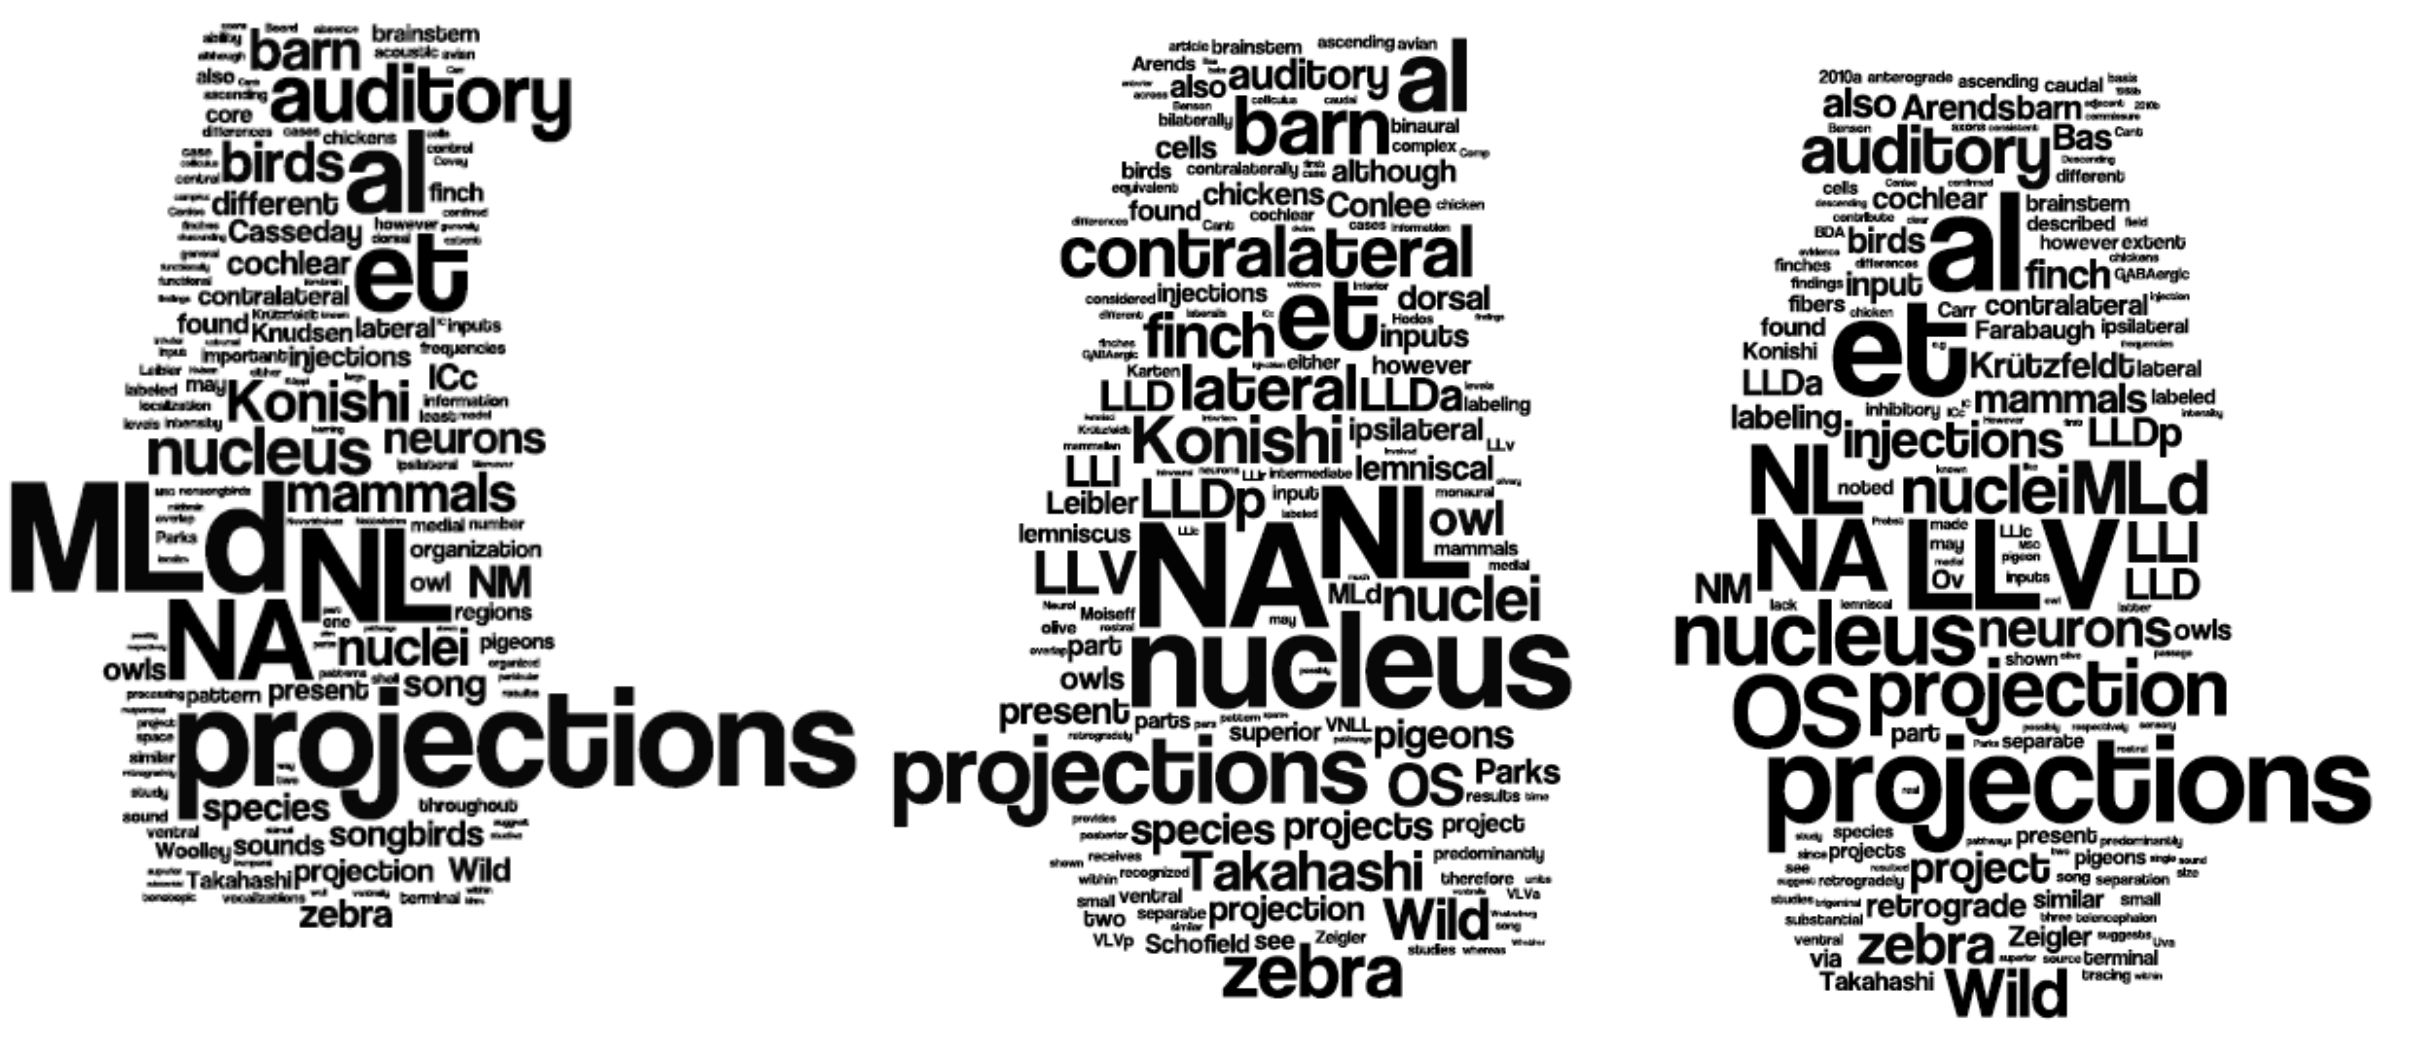
\includegraphics[width=13cm]{Images/Papers-wordle.png}
		\caption{
		{\bf Redundancy in journal articles.} A \href{http://www.wordle.net}{Wordle} from three articles (Kr{\"u}tzfeldt et al 2010a, b and Wild et al 2010) showing the occurrence of individual words in the introduction and discussion sections
		}
		\label{Figure:Wordle}
	\end{center}
\end{figure}


Multiple and sometimes simultaneous discoveries characterise science (Merton 1957, 1963). In a climate where publishing in �high impact factor� journals is a priority~-- and where these journals only publish �novel� findings on a first-come-first-serve 
basis~-- researchers find themselves trying to balance the ethos of scientific openness and collaboration and the need for 
secrecy prior to publication. Some of these issues could be ameliorated by alternative publishing models that allow new data to 
be incorporated to new or to existing published artefacts that appropriately attribute the authors.

\subsection{The situation now}

The rate of increase in the number of groups dedicated to specific areas of research and the accelerated pace at which data can 
be acquired and analysed due to technological and computational advances will probably continue into the future. The burden of 
the peer review system on individual researchers (who provide this service free of charge and for which they receive little credit) 
is becoming increasingly heavier. Further, as research becomes more and more interdisciplinary it is increasingly unlikely that a 
single researcher would be able to critically examine the range of methodologies that are usually included in a single 
multidisciplinary research report.

The value of the traditional scientific article as the primary source of research dissemination must be brought into question. 
Researchers have historically been early and eager adopters of new technology, especially when it accelerates the gathering or 
analysis of data, that is, when it increases productivity. In contrast, the publishing system has remained virtually unchanged since 
its inception. Scientific publications have not shown much innovation aside from the opportunity to publish media (e.g., audio and 
video) that cannot by their very nature be published on paper. Fundamentally, how readers interact with the published article 
(and how the authors interact with the readers) remains virtually intact despite the new possibilities associated with web 2.0 tools 
and the rise of social networks.

\subsubsection{What do we value in a journal?}

\citet{guedon2001ols} described scientists as Dr Jekyll and Mr Hyde. As scientists-authors we are eager to submit our work to high-impact factor journals, but as scientists-readers complain when our libraries cannot afford subscribing to them. What do we then value in journals?

\begin{quote}
�Scientists often care less about the journal title than the ability to track down quickly the full text of articles relevant to their interests. Increasingly, users view titles as merely part of hyperlinked 'content databases' made up of constellations of journal titles.� Butler, 1999
\end{quote}

I would love to meet a scientist that has never uttered the phrase �I cannot believe that got published in Nature� or �I cannot believe that could not get into Nature�. 
%I think I qualify
As scientists-readers we are able to dissociate the value of the science within an article from the perceived value of the journal. If the value of our own work was not measured by the journal in which it is published, what would we value most in a journal?

Before the internet, searching through indexes such as the Current Contents index booklet was tedious and time-consuming and 
when obtaining a copy of an article required sending a �reprint request� postcard to the author (and hope it wouldn�t get lost in the 
mail). Publishing in high impact journals made a difference. The articles had a better chance of being discovered and the 
chances of the journal issues being placed in the �recent arrivals� section of the library were higher. In 1997 the MEDLINE 
database was made available via the internet through PubMed (Weiner 2007). Access to the indices from personal computers 
made it easy to find articles related to a topic, regardless of which journal they were published in. A quick email to an author 
today gets us a pdf copy of the article if this is not available through our libraries. Having lowered the discovery and access 
barriers to articles it is not clear what the impact factor of a journal provides to authors other than the rewards associated with 
assessment. And as long as this continues to be the case, scientists-authors and scientists-readers will continue to be Dr Jekyll 
and Mr Hyde.

In 1991, Paul Grinsparg created the Los Alamos physics archives, a place where scientists could deposit their work, and which 
became a primary resource in the field (Butler 1999). The success of this alternative form of making research results public  
reflects a community that the �work� over the �brand�. But in many disciplines, self-archiving has not gained enough momentum to 
replace traditional publishing. The question is then, what attributes should a publications system need to have to attract both the 
scientist-writer and the scientist-reader? What added value should this new system provide?

The 21st century has seen a rise in the number of researchers that reflect upon whether science is best served by continuing with 
traditional publishing practices. How can we retain the value of the process of scientific communication and peer review but also 
take advantage of the technology that has the potential of accelerating (and enhancing) the way in which scientists communicate 
their results? We have successfully embraced the use of technology to accelerate the generation of data but lagged behind in 
adopting it to accelerate the communication of these results.

\subsubsection[Can we bridge the gap?]{Can we bridge the gap between the cycle of scientific knowledge and the publication cycle?}

%An image (which?) of the research cycle should come somewhere near here.

A good understanding the cyclical and dynamic nature of science is crucial for those incorporating scientific findings into 
educational curricula or evidence-based policies. Scientific knowledge emerges through a series of cycles that begin at the 
conception of an idea and lead to communicating the results. At this point feedback from other scientists helps refine and re-
define the validity and implications of the findings leading to a new iteration of the research cycle where these new possibilities 
are explored. Research is therefore a continuous series of cycles where new findings are first put into old contexts and then integrated into new ones through the emergence of new data. Yet the ways in which scientific findings are reported do not reflect 
this dynamic nature due to the static format of the traditional reporting media nor do they provide an efficient way by which to re-
examine the results in the light of new findings. Imagine two groups simultaneously working on a particular research question 
using two different methodologies, each reaching contradictory conclusions, and both publishing their results at the same time. 
Unaware of each other�s work, the published reports would not cite each other nor consider the implications of each other�s 
contradictory results. Under the current publishing system, these two sets of data could not be easily (and publicly) integrated into 
a new interpretation unless a third publication is produced. As a result, published reports become static snapshots of a single 
research group�s set of experiments that sit isolated from useful discussions that have the potential of re-contextualising the work 
to generate new knowledge. 

Openly licensed scientific literature has the potential of changing the way we interact with the scientific reports. Creative 
Commons licences that allow the content to be distributed and reused offer the potential to modify published reports and adapt 
them in light of new findings. Creative Commons licences (with the exception of those with an ND clause) allow interested parties 
to place original or modified versions of articles where specialists can comment on the methodologies or interpretation of the 
results and where the actual text of the article can be modified. The scientific article in this way can potentially become a living 
document that continues to evolve in parallel with the scientific field of knowledge. 

\subsubsection{What should the next move be?}

Literature that is placed in open collaborative environments can be subjected to post-publication peer review and open 
discussions offered by experts. These discussions can be centred on the entire document or smaller elements within it. 

The individual paper distributed by journals continues to mostly follow the format designed for print - even when journal also 
have online versions. Seldom does the online version add value: corrections cannot be made directly on the article, specialists 
identifying flaws with the methodology are unable to share their views through comments, and new interpretation of the data 
based on new findings cannot be incorporated into the original work. Errors (conceptual or factual) in the original text are often 
perpetuated in subsequent articles.

In 1995 the group led by Eric Kandel (now a Nobel Prize winner) published a paper in Science (Grant et al 1992). Their results 
were challenged by a separate group (Huerta et al 1996). A Google Scholar search shows that the original paper has been cited 
724 times. Of these 724 citations, 533 occurred after1997, after the challenging article had been published, and there were 5 
citations in 2011 at the time of writing this. In contrast, the challenging article by Huerta et al. has only been cited 22 times since it 
was published. The original paper was never retracted, and no opportunities to reconcile the two contradictory findings were 
provided by the publishers. This example highlights how challenged results continue to propagate in the literature and why a 
new way of interacting with the scientific literature is imperative. 

\begin{quote}
�[�] when we assume that people are selfish we build systems that reward selfish behaviours� Clay Shirky (2010)
\end{quote}

Unfortunately, as long as the assessment systems continue to use publication metrics as a proxy for quality these issues cannot be properly addressed. The ubiquitous linking of research quality to publication frameworks (and their rules) provides very few incentives for researchers to contribute to the scientific flows outside of the traditional formats since they do not immediately translate to peer-recognition and are therefore not part of the reward system. 

\subsubsection{What do we propose?}

\begin{quote}
�When you get the right combination of motivations and incentives you change the way that people interact with each other in fairly fundamental ways� Clay Shirky (2010)
\end{quote}

We propose that placing articles in online formats that have a way of tracking individual contributions will lead to a mode of interacting with the literature which will:

\begin{enumerate}
	\item Prevent the dissemination of erroneous facts that arise from typos or omissions
	\item Clarify methodological issues that may be inadequately or incompletely represented in the article
	\item Challenge the validity of the articles through post-publication peer review
	\item Allow the incorporation of orphaned data from other groups that may enhance or contribute to the published article
	\item Incorporate new findings to the interpretation of the presented results (i.e., continuous updating)
\end{enumerate}

Once the articles are placed in these dynamic formats they can become living documents that work in parallel with the scientific community. At the moment, any enhancement (or criticism) of any article continues to occur at lab meetings, journal clubs, etc. These online platforms would allow having these discussions in open forums that are blind to geographic or temporal barriers. The resulting discussions will form an integral part of the scientific work � the author and reader become reader-author and author-reader.

In a more general sense, these platforms have the potential of creating broader benefits. There are several uses for such aggregates that can potentially have a wider impact. 

\begin{enumerate}
\item Health articles about specific regional diseases can be translated and delivered to the local communities where they will have their most impact
\item General articles can be enhanced by accompanying plain English summaries that can be used by science reporters and educators as OERs. 
\item Museums could use these articles to link to them enhancing digital collections. 
\end{enumerate}

Knowledge is deeply rooted in context and collaboration. We propose that publication systems should be built so that they facilitate and encourage the expression of those attributes. A record of the context and collaboration is the centre stone of the preservation of the cultural heritage of science. 



%\subsection{Project description}

%\subsection{Background}
\section{Scientific practice in light of the interactive web}
\label{section:intro2}
{\it An alternative structure for the introduction is outlined in \href{https://github.com/Daniel-Mietchen/Open-Research-Proposals/blob/1c101eb017c9bcb2a8ec72932eff36085bf64590/open-drafting.tex}{this version}. See also section \ref{section:intro} as well as \href{http://en.wikiversity.org/wiki/Wikis_in_scholarly_communication#Comparison_between_paper-based_and_wiki-based_scholarly_communication_systems}{this comparison of paper-based and wiki-based research publishing}.}

Scientific research consists of collaboratively exploring and pushing the boundaries of human knowledge through 
well-documented and contextualized sets of observations. New research results are shared with the scientific 
community, such that their interpretation can be reviewed in the context of existing scientific knowledge, infrastructure 
and methodologies as well as of gaps therein, ultimately leading to new research. 

This sharing of information takes place in the cultural contexts of our global society, and over the last two decades, 
it has moved almost entirely onto the web. In the following, we shall highlight some of the key aspects of communicating research, and how they could be~-- or already are~-- affected by taking place on the interactive web.

%\section{Key aspects of research}
\subsection{Context of existing knowledge}
Relevant for all steps of the research cycle, though typically neglected when actually generating data. Currently distributed over a myriad of articles in thousands of journals that make it practically impossible to keep track of relevant developments outside a very narrow area, and very hard to find out whether some specific research question has already been addressed. Plus access barriers, synonyms and inconsistent usage of terms.

\subsubsection{Duplication of effort}

A lot of projects are being started because (a) the respective researchers are not aware of each other's work, due to inefficient ways of identifying who works on what, and to the secrecy in most fields of research, (b) even if the individual teams were aware of each other's activities, the current highly competitive environment does not provide them with incentives to work together instead of reinventing the wheel, and in some of the few cases where they would try, the disciplinary and national boundaries of research funding effectively prevent that. 

\#\#\# perhaps worth mentioning, if only for some of the numbers involved: \href{http://coburn.senate.gov/public/index.cfm/2011/5/dr-coburn-releases-new-oversight-report-exposing-waste-mismanagement-at-the-national-science-foundation}{this US Republican report has a section on duplication of effort from the side of US funding agencies} \#\#\#

\#\#\# The following subsections are currently just outlines of what could go in there. The order is also likely to change. Only some parts of section \ref{section:intro} will fit in. \#\#\#

\subsection{Ethics}
Typically dealt with at an institutional level, behind closed doors. Reported to the public more or less in a binary fashion (has been approved by the IRB).

\begin{itemize}
	\item informed consent
	\item privacy of certain kinds of data (personal information, location of endangered species etc.)
	\item animal experiments
	\item outright fraud or data manipulation
\end{itemize}

\subsection{Materials and instrumentation}
Hard but not impossible to share. Example: \href{http://www.personalgenomes.org/}{Personal Genome Project}, remote-controlled telescopes.

\subsection{Budget}
Seriously under review as part of the funding application process, little oversight during the research, some review following reports to funders, no review from the wider scientific community.

\subsection{Protocols}
Can be easily shared, but strong links to ethics, materials and instrumentation usually imply that different variants will be in use, even though there might be just a single formal publication.
 
\subsection{Code}
Standard is to report algorithms in mathematical notation or pseudocode, though making code available is more and more popular, and indeed a requirement with some journals or conferences.

Typical problems: Cross-platform interoperability, web-based version, long-term maintainability.

\subsection{Data}
Typically, a publication only provides a summary of the data acquired, and not necessarily of all of it - negative results
in particular remain underreported.

\subsection{Peer review}
In the present system, it acts at three levels - grant peer review decides whether a project is to be funded, journal peer review  whether an article is to be published, and post-publication peer review determines the long-term value and impact of the research reported in the article.

Peer review takes place very rarely when it matters most - when the details of the research are being determined, controls selected and so forth. But that is when it would be most helpful to have insightful commentary (cf. Polymath project).

Similar for data analysis and interpretation.

Pre-publication peer review is slow.
% See also http://rsa.cwrl.utexas.edu/node/5240

\subsection{Outreach}
Currently limited to "scientists say" stories - could be "let's see how they are trying to find out" stories instead, or in addition.

See also \href{http://psych-your-mind.blogspot.com/2011/06/why-we-watch-reality-tv.html}{Why we watch reality TV}

\subsection{Reputation}
Reputation of a researcher is currently mainly determined on the basis of the articles they have published (how many, in which 
journals, oh and about what topic, using which methodology, with what results?) and the amount of grant money they have been
awarded (typically on the basis of their article-based reputation).

Incidentally, these are the two steps in the research cycle that have traditionally involved formal peer review. Wouldn't it thus make sense to assume that allowing for peer review at additional steps in the cycle would provide for additional reputation systems to develop?

This way, the reviewed would gain new dimensions of reputation, and their research would get better if feedback is suitably structured.

\subsection{Discoverability}
Even a very comprehensive search of the formally published literature does not provide a guarantee that all relevant research (even that part that eventually ended up published) will be found.

An encyclopaedic structure (with redirects for synonyms, and disambiguation for homonyms) has discoverability built in. Semantic enhancements would increase it.

\subsection{Discourse}
As \#arseniclife has demonstrated, blogs can be much faster and way more efficient than traditional discourse
See also the \href{http://scienceblogs.com/catdynamics/2009/08/how_to_publish_a_scientific_co.php}{123 steps to publishing a comment} (or \href{http://slawekk.wordpress.com/2010/05/21/how-to-publish-counterexamples-in-1-2-3-easy-steps/}{counterexample})

\subsection{Notes}

\begin{itemize}
	\item record research as it happens
	\item review how it happened
	\item review the interpretation of research results in the context of existing knowledge
	\item identify gaps in knowledge, infrastructure or methodology
	\item stimulate further research
	\item stimulate public engagement
	\item deliver useful outcomes in local and global communities
\end{itemize}

\paragraph{Science in the age of the interactive web}

Every step within the research cycle can in principle be published, not just the ``final'' result.

The project aims at a bit of all of these:
\begin{itemize}
	\item Encyclopaedia of original research
	\item Science as a wiki - i.e. collaboratively updatable database of interlinked articles
	\item GitHub for Science - distributed version control (recent \href{http://bacpathgenomics.wordpress.com/2011/06/13/e-coli-data-released-under-creative-commons-0-license/}{example}: \href{https://github.com/ehec-outbreak-crowdsourced/BGI-data-analysis/wiki}{E. coli O104:H4 analyses on GitHub}); problem to solve: WISIWYG for Git (otherwise wider adoption unlikely)
	\item CC-BY - reusably licensed; forkability
	\item Lab notebook - science as it happens, rather than "scientists found out"
\end{itemize}

Perhaps best to use the above shorthands as titles for the sections of the aims and goals section?
	
%\section{Precursor projects}
\paragraph{Encyclopaedias}
\begin{itemize}
	\item Encyclopaedia Britannica, Wikipedia, Scholarpedia
	\item review articles
\end{itemize}

\paragraph{Lab notebooks}
\begin{itemize}
	\item OpenWetWare
\end{itemize}

\paragraph{Version control}
%restrict description to scholarly publishing
\begin{itemize}
	\item Centralized version control (SVN, CVS)
	\item Distributed version control (GitHub, Mercurial, Bazaar)
\end{itemize}

\paragraph{Collaboratively editable databases}
\begin{itemize}
	\item most wikis, especially Wikipedia
	\item many scientific databases, like GeneBank
	\item Images from \href{http://www.ncbi.nlm.nih.gov/pmc/tools/openftlist/}{PMC OA subset} already being uploaded to \href{http://figshare.com/}{Figshare} (recently reviewed by \href{http://dx.doi.org/10.4103/0976-500X.81919}{\citep{singh2011f}})
\end{itemize}

\paragraph{OA-to-wiki export}
\begin{itemize}
	\item images and taxon treatments from ZooKeys/ Plazi to Species ID and Wikispecies
	\item images from PMC to Figshare
\end{itemize}

\paragraph{Semantic enhancement}
\begin{itemize}
	\item Semantic MediaWiki
\end{itemize}

\paragraph{Reputation system}
\begin{itemize}
	\item StackOverflow
\end{itemize}

\paragraph{Notes}
Room for "fishing expeditions" (data-driven research not directed at particular hypotheses; cf. \href{http://dx.doi.org/10.1091/mbc.E09}{\citep{botstein2010d}}) in addition to hypothesis-driven research

\section{Aims, goals and objectives}
{\it See also \href{http://species-id.net/wiki/Draft:Encyclopaedia_of_original_research#Aims,_Goals_and_Objectives}{the draft over at Species ID}}

\subsection{Turning science into a wiki to make research communication more efficient}
We want to render scientific information more efficient by adapting it to the age of the Web. Specifically, we want to explore the potential of openly licensed scientific information to provide a basis for systematic reuse both within and beyond research contexts. 
\subsubsection{Encyclopaedic structuring of knowledge instead of flood of journal articles}
\href{http://nextbison.wordpress.com/2011/05/18/should-you-believe-wikipedia/}{``So what would you rather have?something checked by three experts over six months to a year, or something checked by 1,727 people in the first 100 hours?  [..]  Also remember that the refereed journal article is fixed at a moment in time, and beyond that any errors or new developments aren?t included.''} - see also \href{http://nextbison.wordpress.com/2011/05/18/should-you-believe-wikipedia/#comment-486}{this comment}

\href{http://opencontract.org/}{early mention of "science as a wiki"}

\subsubsection{Collaborative updatability}
\subsubsection{Forkability}
\subsubsection{Contextualization of research findings}
Paves the way for {\bf Journal of Research Proposals} (\href{http://iphylo.blogspot.com/2011/06/would-you-give-me-grant-experiment-in.html}{demo}) and {\bf Journal of Science Contests}

\subsubsection{Semantic enhancements}
\subsubsection{Reputation schemes compatible with collaboratively edited versioned documents}
See \href{http://www.science3point0.com/evomri/2011/04/16/citing-versioned-papers-robots-and-reviewers/}{this blog post}

\subsubsection{Major hurdles to overcome}
Traditional publications do not reflect (nor have they room for) the continued updating and revising of the published material. This contradicts the nature of science where ideas and results are under constant revision and where interpretation of results are adaptable to new findings. 

Furthermore, even if research communication would take place in a versioned encyclopaedic environment as envisaged here, integration of non-versioned legacy publications still provides a number of challenges, even if they are already digitized and \href{http://blog.datadryad.org/2011/02/22/archiving-legacy-data-or-why-is-dryad-better-than-a-floppy-disk/}{their data made available}.

\subsection{Illustrating the potential of open licenses for reuse in new academic contexts}
\href{http://altmetrics.org/workshop2011/neylon-v0/}{Re-use as a measure of impact}
\href{http://www.earlham.edu/~peters/fos/newsletter/06-02-11.htm}{``When PubMed Central has permission from the copyright holders, it makes articles libre OA and allows bulk downloading.  It calls this the Open Access Subset of PMC. 
http://www.ncbi.nlm.nih.gov/pmc/tools/openftlist/ But only 10\% of PMC belongs in the libre OA subset.  The other 90\% is gratis OA, not libre, and PMC is obliged by the rights-holders to block bulk downloading.  (Thanks to PMC's Ed Sequeira for these details.) Because BioMed Central offers libre OA to its whole corpus, it can offer its whole corpus for bulk downloading. 
http://www.biomedcentral.com/info/about/datamining/ In this sense, libre OA removes custody barriers that gratis OA may leave in place.  The difference between gratis and libre OA isn't limited to permission barriers; permission barriers can create downstream possession and custody barriers.''}

\subsection{Illustrating use cases of open scientific information beyond scholarly contexts}
\subsubsection[Health on a stick]{Health on a stick~-- medical information for rural areas in the developing world}
\label{section:healthonastick}

\begin{figure}[!h]
	\begin{center}
		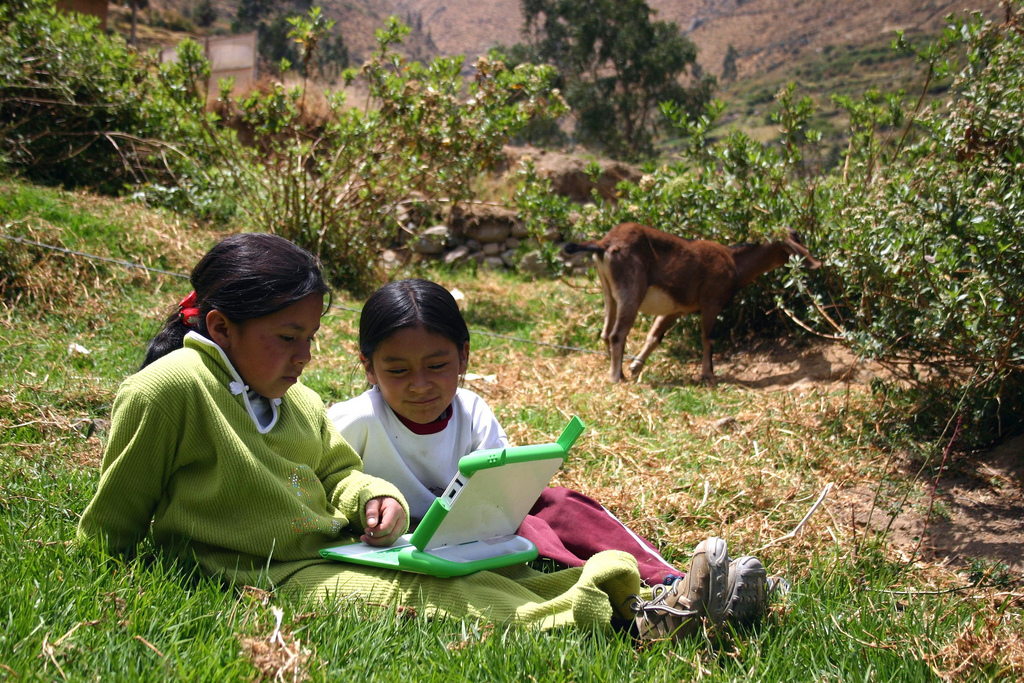
\includegraphics[width=8cm]{Images/Bucolico-full-jpg2png.png}
		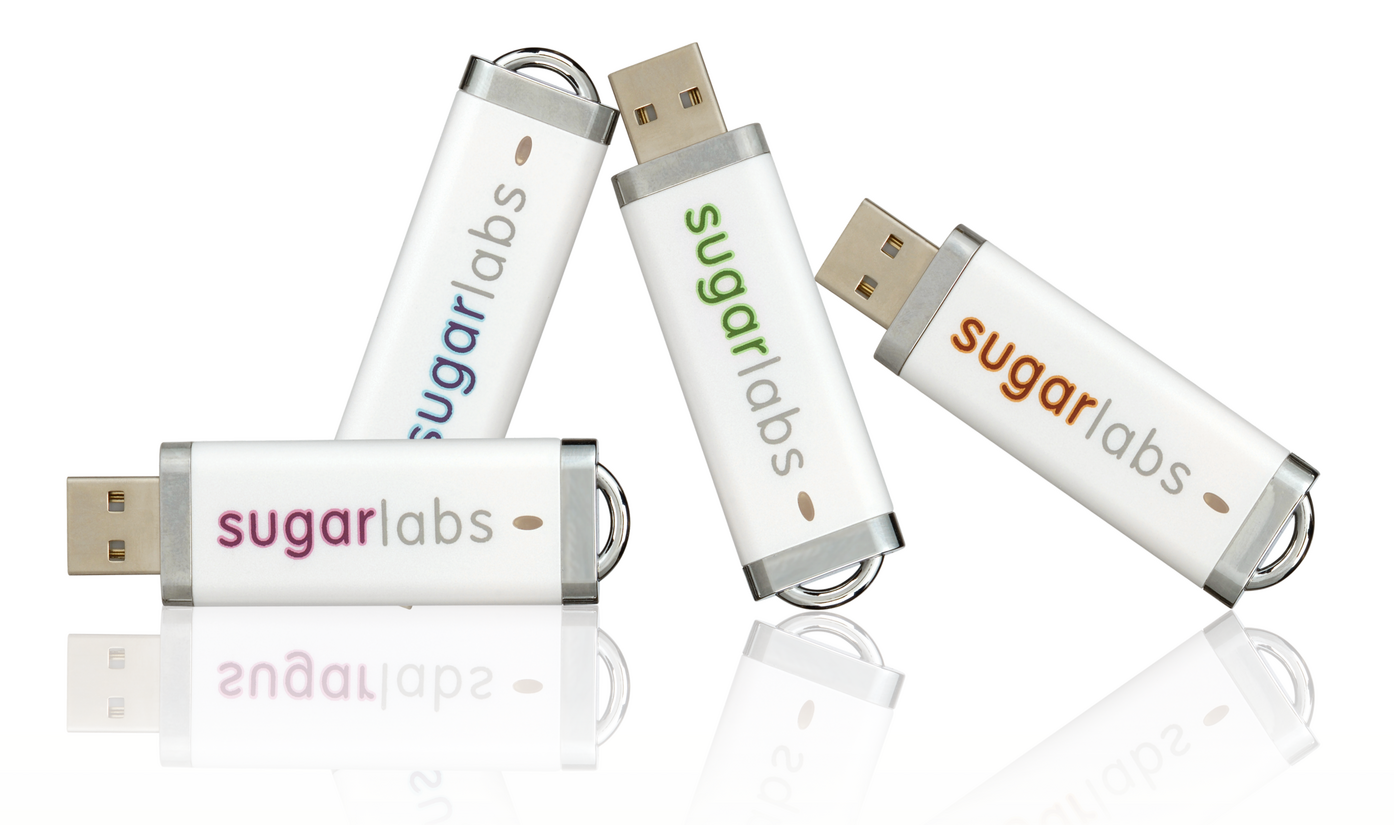
\includegraphics[width=8cm]{Images/SugaronastickMirabelle-cropped.png}
		\caption{
		{\bf Sugar on a stick.} {\bf Left}: The
		\href{http://laptop.org}{One Laptop Per Child  project} (OLPC) project 
		provides children in the developing world with computers,
		so as to support their learning with Open Educational Resources
		and to prepare them for a life in an interconnected world.
		Source: \href{http://wiki.laptop.org/index.php?title=File:Bucolico-full.jpg&oldid=236563}{http://wiki.laptop.org/go/File:Bucolico-full.jpg}. License: \href{http://creativecommons.org/licenses/by-sa/3.0/}{CC-BY-SA}.
		{\bf Right}: 
		\href{http://sugarlabs.org/}{Sugar}~-- 
		the Fedora-based operating system specifically designed for OLPC computers~-- 
		is \href{http://spins.fedoraproject.org/soas/}{available on USB keys} 
		to facilitate development, testing and outreach. 
		Source: \href{http://wiki.sugarlabs.org/index.php?title=File:SugaronastickMirabelle.png&oldid=52111}{http://wiki.sugarlabs.org/go/File:SugaronastickMirabelle.png}. License: \href{http://creativecommons.org/licenses/by/3.0/}{CC-BY}.
		We want to create a variant of 
		such sticks that hosts medical information distilled 
		from the Encyclopaedia of original research in a way compatible with inclusion in OLPC depoyments.
		}
		\label{Figure:Sugaronastick}
	\end{center}
\end{figure}


This subproject is concerned with medical information contained in the Encyclopaedia of original research, which shall be distributed to rural areas in the developing world. 

The word "encyclopaedia" originally referred to a collection of contemporary knowledge 
curated for the same purpose that XO laptops were designed for: educating children.
We want to add a spin to this classical educational paradigm and use XO deployments with Health-on-a-stick versions 
of the Encyclopaedia of original research to reach out across age groups in remote populations.


Further thoughts:

\begin{itemize}
	\item \href{http://www.openzim.org}{openZim} for slicing up wikis for offline use; see also \href{http://en.wikipedia.org/wiki/Wikipedia:WikiProject_Wikislice}{Wikipedia's WikiProject Wikislice}
	\item \href{http://lists.wikimedia.org/pipermail/foundation-l/2008-February/038623.html}{distributed version control} via \href{http://wikipediafs.sourceforge.net/}{WikipediaFs} (on something like GitHub)? The documentation states ``For example, it would be possible to use WikipediaFS to perform a massive content migration from an existing site to a Mediawiki''. See also \href{http://zikoblog.wordpress.com/2011/05/29/wikipedia-offline-2/}{other tools for using Wikipedia offline}
	\item language issues
	\item \href{http://wiki.laptop.org/go/WikiPack}{WikiPack}
	\item mention \href{http://www.olpcnews.com/content/education/how_khan_academy_can_help_olpc.html}{How Khan Academy Can Help OLPC} and \href{http://www.hesperian.org/publications_download.php}{Hesperian Foundation}, which already supported \href{http://site.ebrary.com/lib/hesperian/docDetail.action?docID=10411911}{Where there is No Doctor}
\end{itemize}

%possibly useful illustrations
%http://wiki.laptop.org/go/File:Cover-Edit-990x660.jpg
%http://wiki.laptop.org/go/File:Nepal.JPG
%http://wiki.laptop.org/go/File:20091028-100_7483-990x660.jpg
%http://wiki.laptop.org/go/File:Sugar.png
%http://wiki.laptop.org/go/File:Pic_7.jpg (with stick)
%http://wiki.laptop.org/go/File:Olpc-countries-jun-2010.jpg
%http://wiki.laptop.org/go/File:Agya-olpc4.jpg
%http://wiki.laptop.org/go/File:TrackingSensor.jpg
%http://wiki.laptop.org/go/File:20100331-10-03-31OLPCSchoolVisit019.jpg
%http://wiki.laptop.org/go/File:3080618798_726dedf5f2_o.jpg
%http://wiki.laptop.org/go/File:20081031-Artigas-Uruguay.jpg
%http://wiki.laptop.org/go/File:Nancy_with_her_XO_outdide.jpg
%http://wiki.laptop.org/go/File:Drawn_on_Antintorona_blackboard_OLPC_logo.JPG
%http://wiki.laptop.org/go/File:Mongolia.jpg
%http://wiki.laptop.org/go/File:Oceania-beach.jpg
%http://wiki.laptop.org/go/File:Sierra_leone.jpg
%http://wiki.laptop.org/go/File:Serraleao.JPG
%http://wiki.laptop.org/go/File:XO-a-500.jpg
%http://wiki.sugarlabs.org/go/File:XO-menu.png



\paragraph{Potential side project: \href{http://figshare.com/}{FigShare}/ \href{http://www.gbif.org/communications/news-and-events/showsingle/article/new-incentive-for-biodiversity-data-publishing/}{GBIF-IPT} for OLPC} 
Here, kids could upload images and sensor data as they explore their environment; \href{http://dx.doi.org/10.3897/zookeys.89.903}{sample case} (\href{http://www.eurekalert.org/pub_releases/2011-05/pp-snh051711.php}{summary}) for possible scholarly reuse; biodiversity data could be ideal. Also relevant for \#altmetrics.

Previous (manual) slicing of Wikipedia for educational purposes: \href{http://schools-wikipedia.org}{2008/9 Wikipedia Selection for schools} - too much effort to keep doing manually

\subsubsection{Museums of the future}
See also \href{http://museum3.org}{Museum3}
\subsection{Documenting in public the process of writing a grant proposal}
\subsubsection{Collaborative drafting}
\subsubsection{Feedback from the public}

\section{Timeline}

\subsection{Notes}
\begin{itemize}
	\item \href{http://ff.im/D6rQ0}{Discussion of Gantt chart tools}
\end{itemize}

\section{Sustainability of the project}
\subsection{Sustainability of content}
Key aspect: open licensing; starting with CC-BY.
Also important: content curation.

\subsection{Sustainability of code}
Key aspect: open licensing; starting with the \href{http://www.gnu.org/licenses/gpl.html}{GNU General Public License (GPL)} under which Mediawiki is available.

\subsection{Sustainability of platform}
\href{http://www.pawelszczesny.org/2011/03/02/systems-institute-is-officially-supporting-figshare-backstage-story/}{the example of FigShare}

\subsection{Sustainability of proposal}
The whole proposal has been drafted in public, so as to provide an example anyone can use 
to learn or teach about grant writing, to invite others to come up with similar proposals, to test the potential for public pre-submission peer review, and to stimulate the debate about doing science in the open.

\section{Project team}
\subsection{Applicants}
\subsection{Partners}
We have not defined any formal partnerships yet, but the following are amongst those we are considering:
\begin{itemize}
	\item \href{http://www.enspiral.com}{enspiral} - partner for software development
	\item \href{http://www.ncbi.nlm.nih.gov/pmc/}{PubMed Central} - content partner for seeding of the platform with content
	
\end{itemize}

%\section{Project organization}
\section{Description of work}
\subsection{Work packages (subtasks)}
\subsection{Timeline}
\subsection{Deliverables}

\section{Resource requirements}
\section{Budget}
\section{Acknowledgements}
People\\
Anyone who helped in one way or another\\

Tools\\
\LaTeX, GitHub, Wikiversity, Species-ID, Google Docs, any other tools we used.
Creative Commons, P2PU.

\section{References}
%DM: I would actually prefer to use hyperlinks instead of classical endnotes
%perhaps we can go for both
\bibliographystyle{copernicus}
\bibliography{open-drafting} 


\section{Figures}
%This section is only kept separate during the drafting phase. The figures are to be included in the text as flow permits.
\begin{itemize}
	\item \href{http://www.science3point0.com/evomri/2011/06/08/drafting-proposals-in-the-open-entering-illustrations/}{Call for ideas}
	\item \href{http://www.science3point0.com/evomri/2011/06/15/the-blind-men-and-the-elephant-open-science-version/}{three blind men}
	\item the research cycle in a classical variant (publication as the last step) and a web one (continuous publication of the progress of a project)
\end{itemize}

\section{Possibly useful quotes}
{\it See also \href{http://www.science3point0.com/coaspedia/index.php/User:Daniel_Mietchen/Talks/Slides/Quotes}{this collection}.}

\href{http://ragesoss.com/blog/2006/11/20/top-10-reasons-why-academics-should-edit-wikipedia/comment-page-1/#comment-17727}{``Before the wiki revolution, each time science advanced a new generation would bring out a new generation of textbooks. With the wiki revolution the bits of your work that are superseded will be replaced, and as language changes other bits will be rephrased. But those of your words that are still valid for future generations are likely to be read long after other works have come out of copyright.''}

\href{http://blogs.discovermagazine.com/notrocketscience/2011/06/08/the-renaissance-man-how-to-become-a-scientist-over-and-over-again/}{``�Thirty years ago, you didn�t know what was going on in a different field and you did not have Google. It could take you months to figure out that an idea was a good or bad one. These days, you can get a good sense of that in a matter of minutes because information is much more accessible. That�s really, really huge. It makes it much easier to move from one field to another.�''}

\href{http://knowledgeblog.org/}{Knowledge Blog}: "So what could be more fitting than to revamp science through a platform explicitly built to be revised, commented on, and updated?"

\href{http://twitter.com/#!/egonwillighagen/statuses/39097468700336128}{Yesterday I asked one of my students if she knew what an encyclopedia is, and she said, Is it something like Wikipedia?}

\href{http://friendfeed.com/cameronneylon/c476db70/imo-this-is-possibly-single-most-useful-thing-we}{Jason Priem: ``'How cool would it be to fork articles, a la Github''}

\href{http://marciovm.com/i-want-a-github-of-science}{Marcio van Muhlen: ``We need a GitHub of Science.''}

\section{Notes from earlier stages of the drafting process}
%These notes mostly originated \href{http://species-id.net/wiki/Draft:Encyclopaedia_of_original_research}{on the wiki} and will be woven into the proposal or discarded during the drafting process.



*\href{http://www.wired.com/wiredscience/2011/05/free-science-one-paper-at-a-time-2/all/1}{Nice piece by David Dobbs about Jonathan Eisen's attempts to publish his father's papers online} - could be cited on several points, including \href{http://knowledgeblog.org/}{Knowledge Blog} ("So what could be more fitting than to revamp science through a platform explicitly built to be revised, commented on, and updated?") and the \href{http://www.ariadne.ac.uk/issue7/fytton/}{four essential functions of science} that are currently wrapped up in the scientific paper: registration, certification, dissemination, and preservation

Also cites Antonio Panizzi and mentions ADNI and Mendeley ("Many of the metrics and connections between papers aren?t accessible on the desktop, presumably because they require the server?s data and processing power, and finding them on the web interface feels vaguely opaque.").


\subsection{In focus: The encyclopaedia of original research}

. merging research projects, and linking them with each other as well as with the concepts and methods behind them.

<del>and with any info about the giants, on whose shoulders they have been built</del>

<del>*Copying, forking (e.g. of \href{http://species-id.net/w/index.php?title=Draft:Encyclopaedia_of_original_research&diff=prev&oldid=5076}{this draft}), </del>
<del>*Mention "Science as a wiki" (including blog repository) and \href{http://species-id.net/wiki/Wikis_in_scholarly_publishing}{Wikis in scholarly publishing} and \href{http://friendfeed.com/cameronneylon/c476db70/imo-this-is-possibly-single-most-useful-thing-we}{"Towards threaded publications"} </del>
<del>;possibly embed \href{http://vimeo.com/22633948}{Larry Lessig's talk at CERN, 18 April 2011} </del>
<del>:Lessig's talk is licenced under CC-BY; could be used to highlight issues of license stacking and reuse, also with respect to the default license of the EOR</del>

*EOR: \href{http://www.science3point0.com/coaspedia/index.php/Proposals:Wikimedia_Deutschland/2010/Wissenswert/Wissenschaft_als_Wiki/English}{earlier version}


:comment on the EoR being \href{http://www.opendefinition.org/}{open} and on it being a federation of wikis

\subsubsection{Motivation}
Including definition of goal. Follow SMART scheme.

\subsubsection{Aims}

\subsection{Zooming in}
Discuss what could become of the project ideas that won't end up in the final proposal, and how we plan to go about this decision.

\subsection{Zooming out: Testing open vs. traditional science}

*Do we need a \href{http://open-science.pen.io/ manifesto for open science}? (see also Panton Principles and Altmetrics manifesto)

*\href{http://www.quora.com/What-online-tools-do-scientists-wish-existed-to-facilitate-their-work/answer/Marius-Kempe}{What online tools do scientists wish existed to facilitate their work?}\\
:ORCID-coupled cross-platform reputation system\\
:see also \href{http://www.nature.com/news/2011/110511/full/473138a.html}{this Nature News piece}

\subsection{Notes}

\subsubsection{Quotes}
''See also \href{http://www.science3point0.com/coaspedia/index.php/User:Daniel_Mietchen/Talks/Slides/Quotes}{Collection of "science as a wiki" quotes}.''
\begin{itemize}
	\item  Sandra Bajjalieh: "All of these issues, including the trend towards judging scientists on where they publish instead of what they publish, would be solved if NSF/NIH provided and serviced a highly searchable website onto which people posted results as they obtained them. Search engine capabilities make this entirely feasible. The following features would make the system far superior to the current one of publishing in journals. 1. The comments of interested readers would be added to the posting. Thus there would be peer review. 2. Additional data and revisions that respond to comments could be added. 3. Entry time stamps would solve any issues of priority. 4. The number of "hits" and downloads a link got (similar to the information PLoS One provides for each paper) could serve as a measure of it's interest. This solution is so obvious and the benefits so numerous (NIH program directors would have current updates of research progress, no more publication costs, the ability to imbed movies and animations....)that it's really difficult to understand why there hasn't been more of a move to implement it. Do we, as a community, really want a few people regulating the flow of scientific information?" (\href{http://www.nature.com/news/2011/110427/full/472391a.html}{Sandra Bajjalieh})
	
	\item  Paulo Freire: "At the point of encounter there are neither utter ignorance nor perfect sages; there are only people who are attempting, together, to learn more than they now know." 

	\item  Larry Lessig's talk at CERN, 18 April 2011: http://vimeo.com/22633948 (Lessig's talk is licenced under CC-BY) 
:"copyright is a regulation by the state intended to change a regulation by the market; it's an exclusive right, it's a monopoly right, a property right granted by the state which is necessary to solve an inevitable market failure." \href{http://motherboard.tv/2011/4/25/lessig-copyright-isn-t-just-hurting-creativity-it-s-killing-science-video--2}{ ... in a more colloquial nutshell by Alex Pasternack: Copyright isn't just hurting creativity: it's killing science} 
:: Notes: If we get above the din of this battle is that both sides agree that copyright is necessary for creative works - There is a place for sensible copyright policy but, however, not only artists rely upon copyright. Publishers do too rely upon copyright - the economic problem for publishers is different from that for the artists. We've been fighting a battle where copyright is essential but not on science where copyright is not essential. There is a trouble that few see - How accessible is information for the public? What does it mean for info to be available on the internet? It is only freely accessible if you are part of the 'elite'. Here copyright is placed to benefit the publishers - not the authors - no author has a business model that is built around profiting from this copyright. Does this limitation serve any of the purposes of copyright? What is the publishers objective? To disseminate knowledge or to profit from it? 
::JSTOR archive: has become increasingly criticized because of the cost involved in accessing the articles in the archive. 
::Lessig asks: Can we do better? 
::Open access self archiving movement
::Open access publishing movement:
::Some open is free (as in free speech) some open access is free as in you dont pay for it but other copyright rules apply.
::Science Commons: "broader strategy for producing the information architecture that science needs" as per the 4 principles of Open Science (check on site).
	\item Read write creativity / read-write communities
	\item "Sharing is at the core of the architecture of the net"
::Note by Claudia Koltzenburg:  [by whom?] Barbara van Schewick points out: On the Internet architecture level, due to corporatism, "enclosures" are rampant. The principle of network neutrality that characterized the Internet in its beginning, thirty years ago, has been put at risk particularly by profit-making interests of network providers, observes Barabara van Schewick. The effects of this amount to what economists who think in terms of traditional market economy would call a "market failure". Van Schewick holds that we (and the regulators) need to protect the factors that allowed widespread application innovation in the past (modularity, layering and the end-to-end arguments). These factors made for the openness at the core of the Internet until the early 1990s. Van Schewick recommends let users choose, and practice as much 'application agnosticism' as possible. Internet users today are mostly controlled by flatrate offers and application bundles that leave no alternatives to choose from openly. Van Schewick's argument says that users should indeed be allowed to get a sense of how much they need for what they want to do on the internet ??? and yet maintain a predictability of one's bills. -- see Barbara van Schewick. \href{http://mitpress.mit.edu/books/chapters/0262013975intro1.pdf}{Introduction}. In: Internet Architecture and Innovation. Cambridge, Massachusetts/ London, England: MIT Press, 2010, 1-15.  (see also \href{http://p2pfoundation.net/Internet_Architecture_and_Innovation}{Internet Architecture and Innovation}) -- '''''in this vein, what is the "flatrate" in academic/scholarly/scientific publishing today that lures into control?''''' -- Claudia Koltzenburg 12:12, 1 May 2011 (CEST)

	\item "In the academy [..] we need to recognise an ethical obligation [...] which is at the core of our mission which is universal access to knowledge." Entails: work needs to be free (this should be an ethical point) - We do not need (and should not practice) exclusivity about our work. 
	\item models of access that block access except to a paying elite and discourages innovation.

	\item  Dorothea Salo:  \href{http://scientopia.org/blogs/bookoftrogool/2010/09/16/not-hanging-separately/}{"At the risk of sounding all commie and stuff: we work toward a collective openness, or we die off one by one as the business model sustaining us as well as publishers crumbles to bits."}

	\item  Douglas Rushkoff: As soon as a network is in the hands of policy makers and their funders, this network loses its power to effect change. His conclusion is: "Create new forms that exist beyond any authority's ability to grant them protection", The Next Net. 1 March 2011. \href{http://shareable.net/blog/the-next-net}{Shareable} - Sharing by Design. 

Vannevar Bush. As we may think. \href{http://web.mit.edu/STS.035/www/PDFs/think.pdf}{The Atlantic Monthly, 1945}
	\item "There is a growing mountain of research. But there is increased evidence that we are being bogged down today as specialization extends. The investigator is staggered by the findings and conclusions of thousands of other workers - conclusions which he cannot find time to grasp, much less to remember, asthey appear. Yet specialization becomes increasingly necessary for progress, and the effort to bridge between disciplines is correspondingly superficial"
	\item "
Professionally our methods of transmitting and reviewing the results of research are generations old and
by now are totally inadequate for their purpose.:

	\item ". The summation of human experience us being expanded at a prodigious rate, and
the means we use for threading through the consequent maze to the momentarily important item is the
same as was used in the days of square-rigged ships."
	\item "
A record, if it is to be useful to science, must be continuously extended, it must be stored, and above all it
must be consulted"
	\item "Thus far we seem to be worse
off than before - for we can enormously extend the record; yet even in its present bulk we can hardly
consult it. This is a much larger matter than merely the extraction of data for the purposes of scientific
research; it involves the entire process by which man profits by his inheritance of acquired knowledge."
\end{itemize}

\subsection{Draft of actual proposal}
''Use SMART(ER) approach: Specific/ 
Measurable/ 
Agreed/ 
Realistic/ 
Time constrained.''
\begin{itemize}
	\item Mention subprojects
\end{itemize}

\subsubsection{Potential problems}
\begin{itemize}
	\item \href{http://wikimania2011.wikimedia.org/wiki/Submissions/Barriers_and_opportunities_for_expert_participation_in_Wikipedia:_Results_from_a_survey}{Barriers to expert participation}
	\item *\href{http://cameronneylon.net/blog/michael-nielsen-the-credit-economy-and-open-science/}{Giving credit is key}, and if wiki contributions (or any other science 2.0 activities) would be recognized in academic career terms (\#altmetrics; requires \href{http://marciovm.com/michael-nielsen-on-the-future-of-science functional reputation systems}), scientists would be willing to reallocate their time accordingly


	\item '''What does "publishing" mean in a wiki context?''' The current use of the term "publishing" in itself can be taken as an illustration of how commercial codes and practices seeping into academic culture have not been counteracted successfully since the invention of the Web. In academic CVs, research output in print only (and in electronic but non-open access format) still figures as a "publication", even though the meaning of "to publish" as "make generally known" and "disseminate to the public" has seen fundamental and indeed groundbreaking changes with the Web as a publishing platform. Indeed, "the public" itself has changed fundamentally because today, a "publication" can be made accessible on the web '''without''' \href{http://scientopia.org/blogs/bookoftrogool/2010/03/15/battle-of-the-opens/ "a subscription, per-article, or other fee ... by the reader or the reader's proxy (e.g. a library)"}. Had academic institutions been more interested in the benefit offered by such opportunities, publishing openly would be much more widely accepted today. In this light, nothing should be claimed to be a "publication" any longer unless it is open, maybe even '''in the sense of Open publishing''': \href{http://en.wikipedia.org/w/index.php?title=Special:Cite&page=Open_publishing&id=383242580}{"Open publishing is a process of creating news or other content that is transparent to the readers. They can contribute a story and see it instantly appear in the pool of stories publicly available. Those stories are filtered as little as possible to help the readers find the stories they want. Readers can see editorial decisions being made by others. They can see how to get involved and help make editorial decisions. If they can think of a better way for the software to help shape editorial decisions, they can copy the software because it is free and change it and start their own site. If they want to redistribute the news, they can, preferably on an open publishing site."}
\end{itemize}

\subsubsection{Notes}
\begin{itemize}
	\item Wiki stats tools: \href{http://stats.grok.se/en/201101/Magnetic resonance imaging}{Article-level traffic stats}, \href{http://www.trendingtopics.org/page/Magnetic_resonance_imaging}{Trending topics}, \href{http://www.wikirage.com/}{Edit stats}, \href{http://unit1.conus.info:8080/en.wikipedia.stats/}{Edit stats for new pages}
:See also \href{http://adsabs.harvard.edu/myADS/cache/278851069_PRE.html}{MyADS} in astronomy
	\item \href{http://de.guttenplag.wikia.com/wiki/Benutzer_Blog:Mr._Nice/Quo_vadis,_GuttenPlag}{virtuelles Museum}
	\item Museum fish MRI \& Tierstimmenarchiv
	\item \href{http://ff.im/CCtKf}{Micropayments for culture}  - similar \href{http://friendfeed.com/open-science-summit-2010/a3a7a6ca/sciflies-microfinancing-for-science}{for science}
	\item \href{http://chronicle.com/blogs/profhacker/using-google-docs-forms-to-run-a-peer-review-writing-workshop/33107}{using Google docs}
	\item Open Science Games? Any equivalent to open vs. public peer review?
	\item \href{http://friendfeed.com/kubke/ae9078a8/rt-bestgrid-6pm-tonight-streaming-live}{eResearch talk by Mark Gahegan}
	\item \href{http://museumgam.es/ Museum metadata games}, via \href{http://twitter.com/mia_out}{Twitter}
	\item Filipe Cruz, in Skype chat of May 6, at 19:11 - superfabs: there are a few sites dedicated to harboring science papers and journals in digital free for download formats. would be nice to do a list of them atleast, to analyze and figure out how to better complement them? its similar work i think
:Link provided a bit later: \href{http://xdatelier.org/2010/12/11/open-access-repositories/}{http://xdatelier.org/2010/12/11/open-access-repositories/}
	\item More from that chat: Fabiana Kubke 19:20 
@scann Ah, I see - I was thinking about that earlier today - how do I phrase this to say "as a first step we will do this in this area" - I thought concentrating on one specific (I was thinking Chagas would be a good candidate - I am more familiar with some implications)
	\item \href{https://creativecommons.org/weblog/entry/23831}{https://creativecommons.org/weblog/entry/23831}
	\item \href{http://www.jamendo.com/en/creativecommons}{Jamendo} - company based on distributing CC-licensed music
	\item FigShare as virtual museum?
	\item \href{http://dx.doi.org/10.1038/npre.2010.4603.1}{Community building in ecology}
	\item Use case (from \href{}{Wilbanks talk}): \href{http://selventa.com/technology/white-papers}{Reverse Causal Reasoning}
	\item \href{http://www.guardian.co.uk/education/2011/may/22/open-science-shared-research-internet}{Open science article in the Guardian}
	\item \href{http://www.nature.com/news/2011/110223/full/470437a.html}{"open-access repository for all research findings, which would let scientists log their hypotheses and methodologies before an experiment, and their results afterwards, regardless of outcome"}
	\item Bruce Alberts "Our goal as teachers and educators should be to expose our students to the discovery process and to excite them about challenges at the frontiers of knowledge." (B. Alberts, "A Wakeup Call for Science Faculty", Cell, vol. 123, 2005, pp. 739-741. DOI:\href{http://dx.doi.org/10.1016/j.cell.2005.11.014}{10.1016/j.cell.2005.11.014})
	Also: "Old habits die hard, and I have been disappointed to discover that this is especially true in academia.", from the same source
	\item \href{http://wiss-ki.eu/}{Wiss-ki}
	\item couple things to \href{http://orcid.org/}{ORCID}
	\item \href{http://www.jisc.ac.uk/supportingyourinstitution/researchexcellence/researchvisibility.aspx}{Increasing the impact and visibility of your research}
	\item FirstMonday - \href{http://firstmonday.org/htbin/cgiwrap/bin/ojs/index.php/fm/article/view/583/504}{interview with Linus Torvalds on motivations behind open-sourcing Linux}
	\item Note to self: For basic help with GitHub, see \href{http://help.github.com/git-cheat-sheets/}{http://help.github.com/git-cheat-sheets/ } .
\end{itemize}


\section{Potential funding schemes}
\subsection{Calls for proposals}
\begin{itemize}
	\item Ian Sullivan: \href{http://grants.gov/}{http://grants.gov/}  in the US has a comprehensive listing for all grant opportunities open at the federal level
\end{itemize}
\subsection{Funders with good match in scope}
\begin{itemize}
	\item \href{http://www.shuttleworthfoundation.org/}{Shuttleworth Foundation} - \href{http://www.shuttleworthfoundation.org/funding/fellowship-programme/}{Fellowship scheme} (deadline Nov 1, 2011; \href{http://vimeo.com/10401282}{sample fellowship pitch video})
	\item \href{http://www.macfound.org}{MacArthur Foundation} (co-funder of \href{http://www.eol.org/}{Encyclopedia of Life})
	\item \href{http://www.sloan.org/}{Sloan Foundation} (co-funder of \href{http://www.eol.org/}{Encyclopedia of Life})
	\item \href{http://www.moore.org/}{Gordon \& Betty Moore Foundation} (co-sponsor of Beyond the PDF meeting)
	\item \href{http://www.skollfoundation.org/}{http://www.skollfoundation.org/}
	\item \href{http://www.hhmi.org/}{Howard Hughes Medical Institute} (cf.\ \href{http://www.slate.com/id/2293699/pagenum/all/#p2}{How to fund research so that it generates insanely great ideas, not pretty good ones.})
	\item \href{http://www.jisc.ac.uk}{JISC} (cf.\  \href{http://www.jisc.ac.uk/supportingyourinstitution/researchexcellence/researchvisibility.aspx}{Increasing the impact and visibility of your research})
	\item \href{http://www.volkswagen-stiftung.de/}{VolkswagenStiftung}
	\item see also \href{http://p2pu.org/general/supporters}{supporters of P2PU}
	\item \href{http://www.hfsp.org/}{Human Frontiers Science Program}
	\item \href{http://www.hesperian.org/publications_download.php}{Hesperian Foundation}, especially relevant to section \ref{section:healthonastick} (Health on a stick), as they already supported \href{http://site.ebrary.com/lib/hesperian/docDetail.action?docID=10411911}{Where there is No Doctor}
	\item \href{http://www.kauffman.org/about-foundation/foundation-overview.aspx}{Ewing Marion Kauffman Foundation} (``our researchers must determine what we know, commit to finding the answers to what we don�t, and then apply that knowledge'')
\end{itemize}
\subsection{Prizes and competitions}
\begin{itemize}
	\item \href{http://challenge.gov/NIH/132-nlm-show-off-your-apps-innovative-uses-of-nlm-information}{NIH reuse app challenge}
\end{itemize}

\subsection{Microfinancing}
Invite crowd-sourcing, with link to a description of a project already funded by that source and ideally with some overlap to the current proposal. What role do funders have to play in bringing research into the web age?
\begin{itemize}
	\item \href{http://startl.org/}{Startl} - startup support for socially responsible businesses
	\item \href{https://en.bitcoin.it/wiki/Introduction#Preventing_double-spending}{Bitcoin}; \href{http://www.bitcoinplus.com}{option for mining}
	\item \href{http://www.ccc.de/en/updates/2011/kulturwertmark}{KulturWertMark}
	\item \href{http://blog.kickstarter.com/post/5014573685/happy-birthday-kickstarter}{Kickstarter} - could the subprojects perhaps be submitted there, or to similar places (\href{http://www.indiegogo.com/}{indiegogo}, or \href{http://www.rockethub.com/}{rockethub})?

\end{itemize}

\end{document}